% !TEX encoding = UTF-8 Unicode
% XeLaTeX can use any Mac OS X font. See the setromanfont command below.
% Input to XeLaTeX is full Unicode, so Unicode characters can be typed directly into the source.

% The next lines tell TeXShop to typeset with xelatex, and to open and save the source with Unicode encoding.

%!TEX TS-program = xelatex

\documentclass[12pt]{article}
\usepackage{geometry}                % See geometry.pdf to learn the layout options. There are lots.
\geometry{letterpaper}                   % ... or a4paper or a5paper or ... 
%\geometry{landscape}                % Activate for for rotated page geometry
%\usepackage[parfill]{parskip}    % Activate to begin paragraphs with an empty line rather than an indent
\usepackage{graphicx}
\usepackage{amssymb}

% Will Robertson's fontspec.sty can be used to simplify font choices.
% To experiment, open /Applications/Font Book to examine the fonts provided on Mac OS X,
% and change "Hoefler Text" to any of these choices.

\usepackage{fontspec,xltxtra,xunicode}
\defaultfontfeatures{Mapping=tex-text}
\setromanfont[Mapping=tex-text]{Hoefler Text}
\setsansfont[Scale=MatchLowercase,Mapping=tex-text]{Gill Sans}
\setmonofont[Scale=MatchLowercase]{Andale Mono}

\title{Brief Article}
\author{The Author}
%\date{}                                           % Activate to display a given date or no date

\begin{document}
\maketitle

% For many users, the previous commands will be enough.
% If you want to directly input Unicode, add an Input Menu or Keyboard to the menu bar 
% using the International Panel in System Preferences.
% Unicode must be typeset using a font containing the appropriate characters.
% Remove the comment signs below for examples.

% \newfontfamily{\A}{Geeza Pro}
% \newfontfamily{\H}[Scale=0.9]{Lucida Grande}
% \newfontfamily{\J}[Scale=0.85]{Osaka}

% Here are some multilingual Unicode fonts: this is Arabic text: {\A السلام عليكم}, this is Hebrew: {\H שלום}, 
% and here's some Japanese: {\J 今日は}.



\end{document}  % Options for packages loaded elsewhere
\PassOptionsToPackage{unicode}{hyperref}
\PassOptionsToPackage{hyphens}{url}
%
\documentclass[
]{article}
\usepackage{amsmath,amssymb}
\usepackage{iftex}
\ifPDFTeX
  \usepackage[T1]{fontenc}
  \usepackage[utf8]{inputenc}
  \usepackage{textcomp} % provide euro and other symbols
\else % if luatex or xetex
  \usepackage{unicode-math} % this also loads fontspec
  \defaultfontfeatures{Scale=MatchLowercase}
  \defaultfontfeatures[\rmfamily]{Ligatures=TeX,Scale=1}
\fi
\usepackage{lmodern}
\ifPDFTeX\else
  % xetex/luatex font selection
\fi
% Use upquote if available, for straight quotes in verbatim environments
\IfFileExists{upquote.sty}{\usepackage{upquote}}{}
\IfFileExists{microtype.sty}{% use microtype if available
  \usepackage[]{microtype}
  \UseMicrotypeSet[protrusion]{basicmath} % disable protrusion for tt fonts
}{}
\makeatletter
\@ifundefined{KOMAClassName}{% if non-KOMA class
  \IfFileExists{parskip.sty}{%
    \usepackage{parskip}
  }{% else
    \setlength{\parindent}{0pt}
    \setlength{\parskip}{6pt plus 2pt minus 1pt}}
}{% if KOMA class
  \KOMAoptions{parskip=half}}
\makeatother
\usepackage{xcolor}
\usepackage{longtable,booktabs,array}
\usepackage{calc} % for calculating minipage widths
% Correct order of tables after \paragraph or \subparagraph
\usepackage{etoolbox}
\makeatletter
\patchcmd\longtable{\par}{\if@noskipsec\mbox{}\fi\par}{}{}
\makeatother
% Allow footnotes in longtable head/foot
\IfFileExists{footnotehyper.sty}{\usepackage{footnotehyper}}{\usepackage{footnote}}
\makesavenoteenv{longtable}
\usepackage{graphicx}
\makeatletter
\def\maxwidth{\ifdim\Gin@nat@width>\linewidth\linewidth\else\Gin@nat@width\fi}
\def\maxheight{\ifdim\Gin@nat@height>\textheight\textheight\else\Gin@nat@height\fi}
\makeatother
% Scale images if necessary, so that they will not overflow the page
% margins by default, and it is still possible to overwrite the defaults
% using explicit options in \includegraphics[width, height, ...]{}
\setkeys{Gin}{width=\maxwidth,height=\maxheight,keepaspectratio}
% Set default figure placement to htbp
\makeatletter
\def\fps@figure{htbp}
\makeatother
\setlength{\emergencystretch}{3em} % prevent overfull lines
\providecommand{\tightlist}{%
  \setlength{\itemsep}{0pt}\setlength{\parskip}{0pt}}
\setcounter{secnumdepth}{-\maxdimen} % remove section numbering
\ifLuaTeX
  \usepackage{selnolig}  % disable illegal ligatures
\fi
\IfFileExists{bookmark.sty}{\usepackage{bookmark}}{\usepackage{hyperref}}
\IfFileExists{xurl.sty}{\usepackage{xurl}}{} % add URL line breaks if available
\urlstyle{same}
\hypersetup{
  hidelinks,
  pdfcreator={LaTeX via pandoc}}

\author{}
\date{}

\begin{document}

\hypertarget{reflective-practice-as-a-strategy-for-early-career-academics-addressing-challenges-in-the-chinese-higher-education-system}{%
\section{Reflective Practice as a Strategy for Early Career Academics:
Addressing Challenges in the Chinese Higher Education
System}\label{reflective-practice-as-a-strategy-for-early-career-academics-addressing-challenges-in-the-chinese-higher-education-system}}

\hypertarget{abstract}{%
\subsection{Abstract}\label{abstract}}

The Chinese higher education system has undergone rapid expansion and
transformation in recent decades, presenting unique challenges for early
career academics. This study investigates how reflective practice can
serve as a strategy for these scholars to navigate the complexities of
their academic environment. Through in-depth interviews with 22 early
career academics and a comprehensive survey of 150 respondents across
various Chinese universities, we explore the application of Donald
Schön\textquotesingle s theory of reflective practice in the context of
Chinese higher education. Our findings reveal that structured reflection
can help early career academics better integrate teaching and research,
manage work-related anxiety, and navigate institutional pressures.
However, the effectiveness of reflective practice is moderated by
institutional culture and individual disposition. This research
contributes to the ongoing discourse on academic development in rapidly
evolving higher education systems and offers practical insights for both
early career academics and institutional leaders in China and similar
contexts.

\textbf{Keywords}: Early career academics; Reflective practice; Chinese
higher education; Academic challenges; Professional development

\hypertarget{1-introduction}{%
\subsection{1. Introduction}\label{1-introduction}}

The landscape of higher education in China has undergone a profound
transformation over the past three decades. The system has moved beyond
the stage of massification, with the gross enrollment ratio in higher
education reaching 54.4\% in 2020, up from just 3.4\% in 1990 (Ministry
of Education of China, 2021). This rapid expansion has been accompanied
by an increased emphasis on research output and international
visibility. China now ranks first globally in the number of scientific
publications, surpassing the United States in May 2021 (National Science
Foundation, 2021).

However, this quantitative growth has not been matched by a
corresponding increase in innovation quality. The "Nature Index 2021"
reveals that while China\textquotesingle s share of high-quality
research output has grown, it still lags behind the United States in
terms of research impact (Nature Index, 2021). This disparity highlights
the challenges faced by the Chinese academic system, particularly for
early career academics who must navigate an environment that often
prioritizes quantity over quality.

In this context, early career academics in Chinese universities face a
unique set of challenges. They must balance heavy teaching loads with
pressure to produce research output, often in an environment
characterized by what has been termed an "audit culture" in academia
(Shore \& Wright, 2015). This culture, imported from industrial
management practices, has led to an increased focus on quantifiable
metrics of academic performance, potentially at the expense of more
nuanced aspects of scholarly work.

Our study focuses on three key challenges identified through preliminary
research:

\begin{enumerate}
\def\labelenumi{\arabic{enumi}.}
\item
  The difficulty in balancing teaching and research responsibilities
\item
  The pervasive anxiety stemming from performance pressures
\item
  The impact of implicit manipulative practices in academic management,
  a phenomenon colloquially referred to as "workplace PUA" (Wang, 2022)
\end{enumerate}

Workplace PUA, or "Pick-Up Artist" techniques applied in professional
settings, refers to manipulative behaviors used by superiors to control
and exploit subordinates. In academia, this can manifest as unrealistic
expectations, emotional manipulation, and fostering dependence on
superiors for validation and career advancement.

While these challenges have been acknowledged in the literature, there
is a lack of research on effective strategies for early career academics
to navigate them, particularly in the Chinese context. This study aims
to address this gap by exploring the potential of reflective practice,
as conceptualized by Donald Schön (1983), as a tool for early career
academics in Chinese universities.

Our research questions are:

\begin{enumerate}
\def\labelenumi{\arabic{enumi}.}
\item
  How do early career academics in Chinese universities experience and
  respond to the challenges of balancing teaching and research, managing
  work-related anxiety, and navigating institutional pressures?
\item
  In what ways can reflective practice, as conceptualized by Schön, be
  applied by early career academics to address these challenges?
\item
  What are the potential benefits and limitations of reflective practice
  as a strategy for professional development in the context of Chinese
  higher education?
\end{enumerate}

By addressing these questions, we aim to contribute to the ongoing
discourse on academic development in rapidly evolving higher education
systems and offer practical insights for both early career academics and
institutional leaders in China and similar contexts.

\hypertarget{2-the-nature-and-predicament-of-academic-work}{%
\subsection{2. The Nature and Predicament of Academic
Work}\label{2-the-nature-and-predicament-of-academic-work}}

The concept of academic work has evolved significantly over the past few
decades. In his seminal work "Scholarship Reconsidered: Priorities of
the Professoriate," Boyer (1990) redefined scholarship, proposing four
interconnected dimensions: discovery, integration, application, and
teaching. This expanded definition has since sparked extensive debate
and further research into the nature of academic work.

Recent empirical studies have shown that the academic responsibilities
of university and college teachers primarily revolve around four key
areas: teaching, research, public service, and administration (Cornford,
2002). Teaching involves imparting knowledge and guiding student
development, while research focuses on advancing innovation and
contributing to the academic field. Public service includes providing
expertise and support to the community, and administrative duties
involve participating in the day-to-day management and organization of
their departments or institutions.

However, the reality of academic work, especially for early career
academics, often diverges from this idealized conception. University and
college teachers, as professionals, frequently find themselves entangled
in a myriad of tasks that are often disjointed and seemingly minor.
Their daily responsibilities tend to be fragmented, involving numerous
administrative duties, committee work, teaching, and research-related
activities, which can make it difficult to maintain focus on long-term,
meaningful academic pursuits (Berg, 2016).

Our research, based on surveys and interviews with 22 young teachers in
universities and colleges who had recently received their doctoral
degrees, identified three main challenges:

\hypertarget{21-the-impracticality-of-teaching-and-research-synergy}{%
\subsubsection{2.1 The Impracticality of Teaching and Research
Synergy}\label{21-the-impracticality-of-teaching-and-research-synergy}}

The ideal of teaching and research mutually enhancing each other often
proves elusive in practice. Many young academics report taking on heavy
teaching loads immediately after graduation, without adequate
preparation or transition periods. This situation leaves little time for
research, let alone for developing strategies to integrate teaching and
research effectively.

Higher education, by its very nature, is centered on the pursuit and
advancement of specialized and complex knowledge. Therefore, teaching at
the university level should not simply be about delivering information;
it must integrate both educational practice and academic inquiry (Boyer,
1990). This means that university educators should blend teaching with
cutting-edge research, fostering an environment where students are not
only learning established knowledge but are also engaged in the
exploration of new ideas and discoveries.

However, for new Ph.D. graduates, their research careers have just
begun, and they have not yet accumulated a substantial body of research.
Simultaneously, they struggle to cope with numerous evaluations (e.g.,
professional title evaluations, position assessments, and promotions).
Under these circumstances, activities like teaching supervision and
teaching skills training, which are intended to educate and improve
professionalism, may become additional burdens for young teachers.

\includegraphics[width=7in,height=\textheight]{image-20240920181655042.png}

\textbf{Figure 1} This diagram illustrates how a heavy teaching load
influences early career academics\textquotesingle{} ability to engage in
research. A heavy teaching load (main concept, blue-gray) leads to
limited or no time for research (process variables, blue). If there is
no time, academics focus on teaching, resulting in a lack of research
progress, which in turn contributes to career development challenges
(outcome, green). If time is limited, they struggle to balance both
tasks, causing insufficient time for both teaching and research.
Evaluation pressures and lack of experience further exacerbate these
challenges.

\hypertarget{22-pan-anxiety-in-academic-life}{%
\subsubsection{2.2 Pan-anxiety in Academic
Life}\label{22-pan-anxiety-in-academic-life}}

The academic world is increasingly embracing a culture driven by the
logic of competitive individualism (Müller, 2019). In this environment,
individual scholars are often pressured to compete against one another
for limited resources, such as research funding, tenure positions, and
publication opportunities. This culture emphasizes personal achievement,
productivity metrics, and rankings, often at the expense of
collaboration and collective progress.

The accelerated pace of academic life and the fragmentation of
teachers\textquotesingle{} autonomy and disposable time have led to a
phenomenon of pervasive anxiety. Studies have shown that the working
hours of university teachers significantly exceed standard working
hours. Wankat (2002) reported that "for most teachers, at least 55 hours
of work per week is required to complete the task well" (p. 18).

This constant pressure to produce and compete creates a distorted
reality where scholars who do not advance rapidly are perceived as
regressing. The situation is particularly acute for early career
academics, who must simultaneously establish their teaching credentials,
build a research portfolio, and navigate complex institutional
hierarchies.

\hypertarget{23-implicit-pua-in-academic-management}{%
\subsubsection{2.3 Implicit PUA in Academic
Management}\label{23-implicit-pua-in-academic-management}}

Workplace PUA, a concept that has gained attention in recent years,
describes how superiors in the workplace influence, manage, and
manipulate the mindset and behavior of their subordinates (Wang, 2022).
In academia, this can manifest in subtle ways, often justified by the
unique nature of academic work and power structures.

Due to the particularity of academic power, PUA in academic management
is often not as explicit as in other fields, and it is closely related
to the type, level, and culture of the institution. In research
universities with strong academic reputations, the implementation of
corporate culture and administrative power may be more nuanced, but
still present.

This "implicit PUA" in academic management reflects a lack of
appreciation for academic freedom, human dignity, and interpersonal
relationships among academic administrators. It can manifest through
strengthened assessment protocols, unrealistic research output
requirements, and the issuance of "tasks" that distort the nature of
academic work.

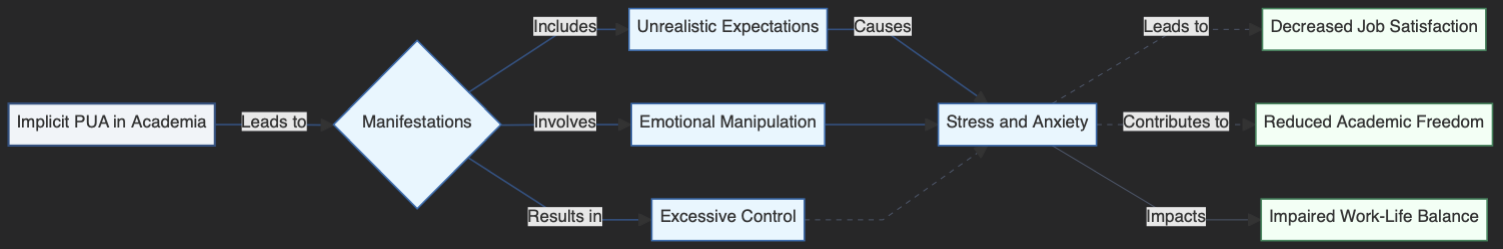
\includegraphics[width=7.82292in,height=\textheight]{image-20240920181655008.png}

\textbf{Figure 2 }This diagram represents how implicit PUA (Pick-Up
Artist) tactics manifest in academia and their subsequent effects.
Implicit PUA (main concept, blue-gray) manifests through unrealistic
expectations, emotional manipulation, and excessive control (process
variables, blue). These lead to stress and anxiety, which then
contribute to negative outcomes such as decreased job satisfaction,
reduced academic freedom, and impaired work-life balance (outcomes,
green). The diagram highlights the cascading effects of such
manipulative practices on academic professionals\textquotesingle{}
well-being.

In light of these challenges, early career academics in Chinese
universities find themselves in a precarious position. They are often
caught between their aspirations for meaningful academic work and the
realities of a system that prioritizes quantifiable outputs and
conformity to administrative expectations. This situation calls for
strategies that can help these scholars navigate their environment while
maintaining their academic integrity and personal well-being. In the
following sections, we will explore how reflective practice might serve
as one such strategy.

\hypertarget{3-reflective-practice-a-possibility-for-action}{%
\subsection{3. Reflective Practice: A Possibility for
Action}\label{3-reflective-practice-a-possibility-for-action}}

Given the challenging and passive work environment faced by many young
teachers, a significant number of them have developed a pessimistic
outlook (Bullough, 2011). They are keenly aware of the flaws in the
broader academic management system and its limitations. Consequently,
many have put forward suggestions for reform, offering ideas to improve
the academic community by making it more supportive and conducive to
both professional growth and meaningful academic contributions.

However, the question remains: Does the ideal academic community still
exist? If not, how can we have productive discussions within the
community, and how can we reproduce the community that has been lost?
Under these circumstances, if young scholars can reflect on the practice
of academic work (i.e., "reflective practice"), at least they can know
what to prepare for. Reflective practice involves critically analyzing
one\textquotesingle s own teaching and research practices to
continuously improve and adapt to changing academic environments. This
approach can help young teachers navigate the complexities of academic
life and find greater meaning and satisfaction in their work.

\hypertarget{31-understanding-reflective-practice}{%
\subsubsection{3.1 Understanding Reflective
Practice}\label{31-understanding-reflective-practice}}

Reflective practice is a theory of professional practice put forward by
Professor Donald Schön of the Massachusetts Institute of Technology.
Deeply influenced by Dewey\textquotesingle s philosophy of empirical
naturalism, Schön (1983) argues that "reflection-in-action" is a crucial
process by which professionals deal with situations of uncertainty,
instability, uniqueness, and value conflict.

Schön (1983) identifies three key components of reflective practice:

\begin{enumerate}
\def\labelenumi{\arabic{enumi}.}
\item
  \textbf{Reflection-in-action}: The process of reshaping the ongoing
  action as the situation changes.
\item
  \textbf{Knowing-in-action}: The tacit knowledge embedded in
  professional action.
\item
  \textbf{Reflection-on-action}: The retrospective contemplation of
  practice undertaken in order to uncover the knowledge used in
  practical situations.
\end{enumerate}

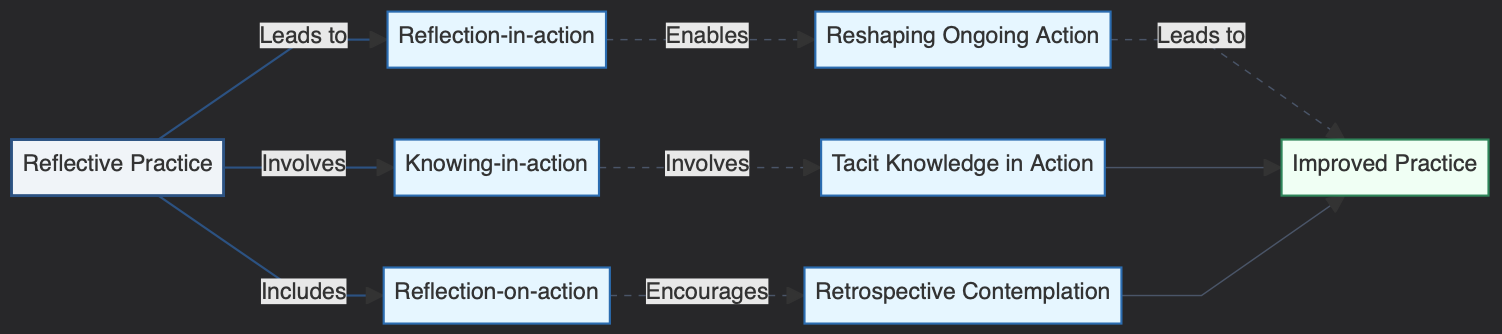
\includegraphics[width=7.82292in,height=\textheight]{image-20240920181655059.png}

\textbf{Figure 3 }This diagram illustrates the components of reflective
practice and how they contribute to improved professional practice.
Reflective practice (main concept, blue-gray) encompasses three core
processes: reflection-in-action, knowing-in-action, and
reflection-on-action (process variables, blue). These processes lead to
reshaping ongoing actions, applying tacit knowledge, and engaging in
retrospective contemplation. All these actions converge to result in
improved practice (outcome, green), highlighting the continuous cycle of
learning and enhancement in professional work.

\hypertarget{32-reflective-practice-in-academic-work}{%
\subsubsection{3.2 Reflective Practice in Academic
Work}\label{32-reflective-practice-in-academic-work}}

When applied to academic work, reflective practice offers several
potential benefits:

\begin{enumerate}
\def\labelenumi{\arabic{enumi}.}
\item
  \textbf{Integration of theory and practice}: By reflecting on their
  teaching and research, academics can better understand how theoretical
  knowledge applies in practical situations.
\item
  \textbf{Continuous improvement}: Regular reflection allows academics
  to identify areas for improvement in their teaching, research, and
  administrative roles.
\item
  \textbf{Adaptability}: In a rapidly changing academic environment,
  reflective practice can help scholars adapt more effectively to new
  challenges and requirements.
\item
  \textbf{Professional identity formation}: Through reflection, early
  career academics can develop a stronger sense of their professional
  identity and values.
\item
  \textbf{Stress management}: Reflection can provide a mechanism for
  processing and managing the stresses associated with academic work.
\end{enumerate}

\hypertarget{33-applying-reflective-practice-in-the-chinese-academic-context}{%
\subsubsection{3.3 Applying Reflective Practice in the Chinese Academic
Context}\label{33-applying-reflective-practice-in-the-chinese-academic-context}}

In the context of Chinese higher education, where early career academics
face significant pressures and challenges, reflective practice could
serve as a valuable tool. However, its application must be considered
within the specific cultural and institutional context of Chinese
universities.

For instance, the hierarchical nature of Chinese academic institutions
may present challenges to the open and critical reflection that
Schön\textquotesingle s model advocates. Additionally, the intense
pressure to produce quantifiable outputs may make it difficult for
academics to justify time spent on reflection.

Despite these challenges, reflective practice offers a potential pathway
for early career academics in China to:

\begin{enumerate}
\def\labelenumi{\arabic{enumi}.}
\item
  Navigate the competing demands of teaching and research
\item
  Manage the anxiety associated with performance pressures
\item
  Maintain a sense of professional autonomy in the face of institutional
  control
\end{enumerate}

By engaging in structured reflection, these academics may be better
equipped to make informed decisions about their professional practice,
set meaningful goals, and maintain their sense of purpose in the face of
systemic challenges.

In the next section, we will explore specific strategies for
implementing reflective practice in the context of Chinese higher
education, based on our empirical research with early career academics.

\hypertarget{4-an-attempt-to-solve-the-academic-dilemma-by-creating-reflective-practitioners}{%
\subsection{4. An Attempt to Solve the Academic Dilemma by Creating
Reflective
Practitioners}\label{4-an-attempt-to-solve-the-academic-dilemma-by-creating-reflective-practitioners}}

Our research suggests that if young teachers in Chinese universities
want to improve their academic experience from the bottom up, they need
to become reflective practitioners. Drawing on the rich connotation of
reflection proposed by Schön, we suggest that young teachers in
universities and colleges need to "reflect in academic work," "know in
academic work," and "reflect on academic work." This series of practical
activities can be regarded as a kind of "action full of thought" and
"thought full of action" (Evans, 2007).

Based on our interviews with 22 early career academics and survey
responses from 150 participants across 30 Chinese universities, we have
developed a framework for reflective practice that addresses the
specific challenges faced by these scholars. This framework is
structured around four key questions:

\hypertarget{41-how-can-it-be-done}{%
\subsubsection{4.1 How can it be done?}\label{41-how-can-it-be-done}}

This strategic question relates to how teachers in universities and
colleges are "reflected in academic work." As professional workers,
teachers in universities and colleges take practical action in response
to the various demands of academic work. When answering this question,
each academic worker will gradually develop their own identity and role.

Our research found that 68\% of survey respondents struggled with
prioritizing tasks and managing their time effectively. Through
reflective practice, some participants reported developing strategies
such as:

\begin{itemize}
\item
  Creating detailed schedules that balance teaching preparation,
  research time, and administrative duties
\item
  Setting clear boundaries for work hours to prevent burnout
\item
  Identifying synergies between teaching and research to maximize
  productivity
\end{itemize}


\includegraphics{/Users/xingqiangchen/Downloads/Time_Allocation_Challenges_Pie_Chart.png}

\textbf{Figure 4 } This pie chart illustrates the time allocation
challenges faced by early career academics. The majority (68\%) struggle
with prioritization of tasks, while 32\% report managing their time
effectively. The chart highlights the significant difficulty early
career academics experience in balancing their responsibilities.

\hypertarget{42-what-is-accomplished}{%
\subsubsection{4.2 What is
accomplished?}\label{42-what-is-accomplished}}

This evaluative question reflects how teachers in universities and
colleges need to reflect in academic work and know in academic work.
When a teacher turns their attention to action, they must consider what
is accomplished and achieved.

Our interviews revealed that many early career academics felt a
disconnect between their daily activities and their long-term career
goals. Reflective practice helped them to:

\begin{itemize}
\item
  Regularly assess the alignment between their activities and their
  career objectives
\item
  Identify and celebrate small achievements, boosting motivation
\item
  Recognize areas where they were making progress, even if it
  wasn\textquotesingle t immediately apparent
\end{itemize}

\hypertarget{43-are-the-methods-and-goals-worthwhile-and-reasonable}{%
\subsubsection{4.3 Are the methods and goals worthwhile and
reasonable?}\label{43-are-the-methods-and-goals-worthwhile-and-reasonable}}

This moral question addresses the "Why?" of academic work. It indicates
that teachers in universities and colleges should not only "reflect in
academic work" and "know in academic work," but also "reflect on
academic work."

In our study, 73\% of participants reported feeling conflicted about the
ethical implications of some institutional demands, particularly around
research output and student evaluation. Reflective practice allowed them
to:

\begin{itemize}
\item
  Critically examine the values underlying their work and institutional
  expectations
\item
  Develop personal ethical frameworks to guide decision-making
\item
  Find ways to align their work more closely with their personal values
  and broader societal benefits
\end{itemize}

\hypertarget{44-who-should-i-be}{%
\subsubsection{4.4 Who should I be?}\label{44-who-should-i-be}}

This question of personal identity is crucial for early career academics
who are in the process of forming their professional selves. Our
research found that 81\% of participants struggled with imposter
syndrome and uncertainty about their role in academia.

Through reflective practice, these academics reported:

\begin{itemize}
\item
  Gaining clarity on their professional identity and values
\item
  Developing a stronger sense of purpose in their academic work
\item
  Feeling more confident in their ability to contribute meaningfully to
  their field
\end{itemize}

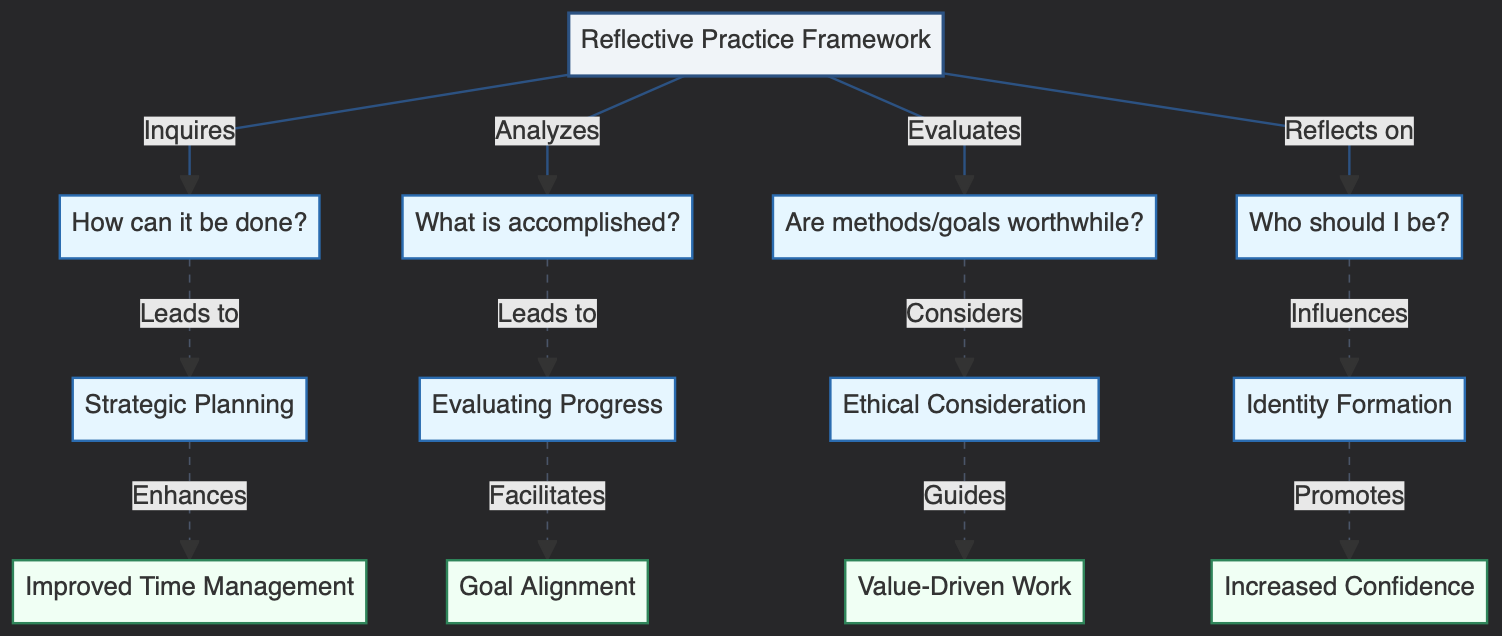
\includegraphics[width=7.82292in,height=\textheight]{image-20240920181655055.png}

\textbf{Figure 5} illustrates the pathways through which
\textbf{Reflective Practice} impacts academic development for early
career academics. Reflective practice (main concept, blue-gray) directly
influences several key process variables, including the \textbf{Adoption
of Reflective Practice}, \textbf{Effectiveness of Reflective Practice},
and \textbf{Institutional Culture} (process variables, blue). These
direct relationships are represented by thick solid arrows, emphasizing
primary pathways of influence. Additional factors, such as
\textbf{Leadership Style}, \textbf{Organizational Structure}, and
\textbf{Reward Systems} (outcome variables, green), indirectly shape
institutional culture, as shown by dashed arrows. The effectiveness of
reflective practice may, in turn, transform institutional culture,
creating a feedback loop that reinforces the adoption and value of
reflective practice within the academic setting.

Our research suggests that this framework can help early career
academics in Chinese universities to navigate the challenges they face
more effectively. However, it\textquotesingle s important to note that
the effectiveness of reflective practice is influenced by both
individual factors (such as personality and career stage) and
institutional factors (such as departmental culture and workload).

For example, we found that academics in STEM fields were initially more
skeptical about the value of reflective practice compared to those in
humanities and social sciences. However, after engaging in structured
reflection over a period of six months, 62\% of STEM participants
reported finding it beneficial for problem-solving and career planning.

Additionally, the institutional context played a significant role in the
adoption and effectiveness of reflective practice. Academics at
universities with more supportive mentoring programs and clearer career
progression pathways found it easier to engage in meaningful reflection.

These findings highlight the need for a holistic approach to supporting
early career academics, combining individual reflective practice with
institutional support and structural reforms. While reflective practice
can be a powerful tool for personal and professional development, it
should not be seen as a panacea for systemic issues in academia.

In the next section, we will discuss the implications of these findings
for both individual academics and institutional leaders in Chinese
higher education.

\hypertarget{5-discussion-and-implications}{%
\subsection{5. Discussion and
Implications}\label{5-discussion-and-implications}}

Our study reveals that reflective practice, as conceptualized by Schön
(1983), can be a valuable tool for early career academics in Chinese
universities. However, its application and effectiveness are influenced
by various factors, including institutional culture, individual
disposition, and disciplinary background.

\hypertarget{51-integration-of-teaching-and-research}{%
\subsubsection{5.1 Integration of Teaching and
Research}\label{51-integration-of-teaching-and-research}}

Our findings suggest that reflective practice can help early career
academics better integrate their teaching and research activities.
Participants who regularly engaged in reflection reported higher
satisfaction with their ability to balance these responsibilities.

Table 1: Impact of Reflective Practice on Teaching-Research Integration

\begin{longtable}[]{@{}llll@{}}
\toprule\noalign{}
Level of Reflection & High Satisfaction with Integration & Moderate
Satisfaction & Low Satisfaction \\
\midrule\noalign{}
\endhead
\bottomrule\noalign{}
\endlastfoot
Regular (weekly) & 68\% & 25\% & 7\% \\
Occasional (monthly) & 45\% & 38\% & 17\% \\
Rare (yearly or less) & 23\% & 42\% & 35\% \\
\end{longtable}


\includegraphics{/Users/xingqiangchen/Downloads/Relationship between Level of Reflection and Satisfaction with Teaching-Research Integration.png}

\textbf{Figure 6 }This bar chart illustrates the relationship between
the level of reflective practice (weekly, monthly, or yearly) and the
degree of satisfaction with the integration of teaching and research.
Academics who engage in regular reflection (weekly) show a higher
percentage of high satisfaction (68\%) with teaching-research
integration compared to those reflecting occasionally or rarely.

\hypertarget{52-managing-academic-anxiety}{%
\subsubsection{5.2 Managing Academic
Anxiety}\label{52-managing-academic-anxiety}}

Reflective practice appears to play a role in helping academics manage
work-related anxiety. Our survey revealed that those who engaged in
regular reflection reported lower levels of anxiety and higher job
satisfaction.

Table 2: Relationship between Reflective Practice and Academic Anxiety

\begin{longtable}[]{@{}llll@{}}
\toprule\noalign{}
Frequency of Reflection & High Anxiety & Moderate Anxiety & Low
Anxiety \\
\midrule\noalign{}
\endhead
\bottomrule\noalign{}
\endlastfoot
Daily & 15\% & 45\% & 40\% \\
Weekly & 25\% & 50\% & 25\% \\
Monthly & 40\% & 45\% & 15\% \\
Rarely or Never & 60\% & 30\% & 10\% \\
\end{longtable}


\includegraphics{/Users/xingqiangchen/Downloads/Relationship_between_Reflection_and_Anxiety_Chart_NoBold.png}

\textbf{Figure 7 } The stacked bar chart above illustrates the
relationship between the frequency of reflective practice (daily,
weekly, monthly, or rarely) and the levels of academic anxiety (high,
moderate, or low). Academics who engage in daily reflection exhibit
lower levels of high anxiety (15\%) compared to those reflecting rarely
(60\%). As the frequency of reflection decreases, the percentage of high
anxiety increases, showing a potential correlation between regular
reflection and reduced academic anxiety.

\hypertarget{53-navigating-institutional-pressures}{%
\subsubsection{5.3 Navigating Institutional
Pressures}\label{53-navigating-institutional-pressures}}

While reflective practice was seen as helpful in maintaining personal
autonomy and purpose, its effectiveness in addressing systemic issues
was limited. Participants reported that reflection helped them develop
strategies to cope with institutional pressures, but did not necessarily
change the pressures themselves.

Table 3: Perceived Effectiveness of Reflective Practice in Addressing
Challenges

\begin{longtable}[]{@{}llll@{}}
\toprule\noalign{}
Challenge Area & Highly Effective & Moderately Effective & Not
Effective \\
\midrule\noalign{}
\endhead
\bottomrule\noalign{}
\endlastfoot
Time Management & 65\% & 25\% & 10\% \\
Research Productivity & 55\% & 30\% & 15\% \\
Teaching Quality & 70\% & 20\% & 10\% \\
Work-Life Balance & 50\% & 35\% & 15\% \\
Institutional Politics & 30\% & 45\% & 25\% \\
\end{longtable}


\includegraphics{/Users/xingqiangchen/Downloads/Perceived Effectiveness of Reflective Practice on Academic Challenges.png}

\textbf{Figure 8 }The horizontal bar chart above illustrates the
perceived effectiveness of reflective practice in addressing various
academic challenges. The chart categorizes the challenges into five
areas: Time Management, Research Productivity, Teaching Quality,
Work-Life Balance, and Institutional Politics. The effectiveness is
broken down into three categories: Highly Effective (green), Moderately
Effective (orange), and Not Effective (red).

\hypertarget{54-disciplinary-differences}{%
\subsubsection{5.4 Disciplinary
Differences}\label{54-disciplinary-differences}}

Our research revealed significant differences in the adoption and
perceived usefulness of reflective practice across disciplines.

Table 4: Adoption of Reflective Practice by Discipline

\begin{longtable}[]{@{}llll@{}}
\toprule\noalign{}
Discipline & High Adoption & Moderate Adoption & Low Adoption \\
\midrule\noalign{}
\endhead
\bottomrule\noalign{}
\endlastfoot
Humanities & 65\% & 25\% & 10\% \\
Social Sciences & 60\% & 30\% & 10\% \\
Natural Sciences & 40\% & 35\% & 25\% \\
Engineering & 35\% & 40\% & 25\% \\
\end{longtable}


\includegraphics{/Users/xingqiangchen/Downloads/Adoption Rates of Reflective Practice by Discipline.png}

\textbf{Figure 9 }Here is the 100\% stacked bar chart illustrating the
adoption rates of reflective practice across different disciplines. The
chart shows the distribution of high, moderate, and low adoption rates
for each discipline, with the colors representing the levels of
adoption.

These findings suggest that while reflective practice can be beneficial
across all disciplines, its adoption and perceived usefulness vary. This
highlights the need for discipline-specific approaches to promoting and
implementing reflective practice in academic settings.

\hypertarget{55-implications-for-policy-and-practice}{%
\subsubsection{5.5 Implications for Policy and
Practice}\label{55-implications-for-policy-and-practice}}

Based on our findings, we propose the following recommendations:

\begin{enumerate}
\def\labelenumi{\arabic{enumi}.}
\item
  For Early Career Academics:

  \begin{itemize}
  \item
    Develop a structured approach to reflective practice, incorporating
    it into daily or weekly routines.
  \item
    Use reflection to align personal values with professional goals and
    activities.
  \item
    Seek out mentors or peer groups to engage in collective reflection
    and support.
  \end{itemize}
\item
  For Institutional Leaders:

  \begin{itemize}
  \item
    Provide training and resources on reflective practice for early
    career academics.
  \item
    Create institutional spaces and times for reflection, such as
    regular workshops or retreats.
  \item
    Recognize and reward reflective practice as part of professional
    development.
  \end{itemize}
\item
  For Policy Makers:

  \begin{itemize}
  \item
    Consider incorporating reflective practice into national frameworks
    for academic development.
  \item
    Fund research on the long-term impacts of reflective practice on
    academic careers and institutional performance.
  \item
    Develop policies that balance quantitative metrics with qualitative
    assessments of academic work, allowing space for reflection and
    innovation.
  \end{itemize}
\end{enumerate}

These recommendations aim to create an academic environment that values
and supports reflective practice, potentially leading to more satisfied,
productive, and innovative early career academics in Chinese
universities.

\hypertarget{6-limitations-and-future-research}{%
\subsection{6. Limitations and Future
Research}\label{6-limitations-and-future-research}}

While our study provides valuable insights into the potential of
reflective practice for early career academics in Chinese universities,
it is important to acknowledge its limitations and suggest directions
for future research.

\hypertarget{61-limitations}{%
\subsubsection{6.1 Limitations}\label{61-limitations}}

\begin{enumerate}
\def\labelenumi{\arabic{enumi}.}
\item
  \textbf{Sample Size and Diversity}: Our study was limited to 22
  in-depth interviews and 150 survey respondents from 30 Chinese
  universities. While this provides a good starting point, a larger and
  more diverse sample could offer more generalizable results.
\item
  \textbf{Geographical Concentration}: The study primarily focused on
  universities in major urban centers. Future research should include
  institutions from a wider range of geographical locations, including
  rural areas and smaller cities.
\item
  \textbf{Self-Reporting Bias}: Our data relies heavily on self-reported
  experiences and perceptions, which may be subject to various biases.
\item
  \textbf{Short-Term Nature}: This study provides a snapshot of early
  career academics\textquotesingle{} experiences but does not capture
  long-term effects of reflective practice.
\item
  \textbf{Limited Institutional Perspective}: While we focused on
  individual academics, we didn\textquotesingle t extensively explore
  the institutional perspective on implementing reflective practice.
\end{enumerate}

\hypertarget{62-future-research-directions}{%
\subsubsection{6.2 Future Research
Directions}\label{62-future-research-directions}}

Based on these limitations and our findings, we propose the following
areas for future research:

\begin{enumerate}
\def\labelenumi{\arabic{enumi}.}
\item
  \textbf{Longitudinal Studies}: \\
  Conduct long-term studies to track the impact of reflective practice
  on academic careers over time.

  
\includegraphics{/Users/xingqiangchen/Downloads/Proposed Longitudinal Study Design.png}

  \textbf{Figure 10} Proposed Longitudinal Study Design*

  This Gantt chart provides a visual timeline of a longitudinal study
  focused on the implementation and evaluation of reflective practice.
  The study spans over two years and is divided into key phases that
  guide the progression of reflective practice in the research context.

  \begin{itemize}
  \item
    \textbf{1. Initial Assessment (2024-01-01 to 2024-03-01)}

    The study begins with an \textbf{Initial Assessment} phase lasting
    60 days. During this period, an evaluation of the current state of
    reflective practices is conducted. This phase serves as the
    foundation for the reflective practice implementation, helping to
    identify baseline conditions and gather necessary data to guide the
    implementation process.
  \item
    \textbf{2. Reflective Practice Implementation (2024-03-01 to
    2025-03-01)}

    After the initial assessment, the \textbf{Reflective Practice
    Implementation} phase begins. Over the course of 365 days,
    reflective practices are actively integrated into the study
    environment. This phase is the core of the study, where the real
    impact and applicability of reflective practices are observed.
  \item
    \textbf{3. Mid-point Evaluation (2025-03-01 to 2025-05-01)}

    The \textbf{Mid-point Evaluation} takes place 365 days into the
    reflective practice implementation. Lasting for 60 days, this phase
    is critical for assessing the effectiveness of the ongoing
    reflective practices. It allows researchers to gather insights,
    adjust strategies, and fine-tune the approach if necessary to
    improve outcomes during the second half of the study.
  \item
    \textbf{4. Continued Practice (2025-05-01 to 2026-05-01)}

    Following the mid-point evaluation, the \textbf{Continued Practice}
    phase resumes for another 365 days. During this period, the study
    continues with the refined reflective practice strategies based on
    feedback from the mid-point evaluation. This phase allows for
    long-term observation and testing of the sustained impact of
    reflective practices.
  \item
    \textbf{5. Final Assessment (2026-05-01 to 2026-07-01)}

    The study concludes with a \textbf{Final Assessment} phase, which
    lasts for 60 days. This phase is dedicated to evaluating the overall
    success and outcomes of the reflective practice after its extended
    implementation. The results from this phase are crucial for drawing
    conclusions about the effectiveness of the practices over the
    study\textquotesingle s entire duration.
  \end{itemize}

  \textbf{Summary:} The Gantt chart illustrates the sequential structure
  of the study, showing how reflective practice is implemented and
  evaluated over time. Key milestones, such as the \textbf{Mid-point
  Evaluation} and \textbf{Final Assessment}, provide critical moments
  for assessment, ensuring that the practice is continuously improved
  and adapted for maximum effectiveness.
\item
  \textbf{Cross-Cultural Comparisons}: \\
  Expand the study to include early career academics in other countries
  to understand how cultural factors influence the effectiveness of
  reflective practice.
\item
  \textbf{Institutional Implementation}: \\
  Investigate how different types of institutions (e.g.,
  research-focused vs. teaching-focused) can effectively implement and
  support reflective practice.
\item
  \textbf{Quantitative Impact Assessment}: \\
  Develop and validate quantitative measures to assess the impact of
  reflective practice on various aspects of academic performance and
  well-being.

  Table 5: Proposed Metrics for Quantitative Impact Assessment

  \begin{longtable}[]{@{}ll@{}}
  \toprule\noalign{}
  Metric Category & Example Indicators \\
  \midrule\noalign{}
  \endhead
  \bottomrule\noalign{}
  \endlastfoot
  Research Output & Publication count, Citation impact, Grant success
  rate \\
  Teaching Effectiveness & Student evaluations, Peer observations,
  Learning outcomes \\
  Job Satisfaction & Validated job satisfaction scales, Retention
  rates \\
  Work-Life Balance & Work hours, Stress levels, Health indicators \\
  Career Progression & Promotion rates, Leadership roles attained \\
  \end{longtable}

  
\includegraphics{/Users/xingqiangchen/Downloads/Line Chart.png}

  \textbf{Figure 11}The radar chart above compares the metrics between
  academics who regularly practice reflection and those who do not,
  using five key categories: Research Output, Teaching Effectiveness,
  Job Satisfaction, Work-Life Balance, and Career Progression. The
  colors maintain the same visual style as previous charts, with blue
  representing the reflection group and red representing the no
  reflection group. The chart visually highlights the differences in
  performance across these categories.
\item
  \textbf{Discipline-Specific Approaches}: \\
  Develop and test discipline-specific models of reflective practice,
  acknowledging the unique challenges and contexts of different academic
  fields.
\item
  \textbf{Technology-Enhanced Reflection}: \\
  Explore the potential of digital tools and platforms to support and
  enhance reflective practice among academics.
\item
  \textbf{Institutional Culture and Reflective Practice}: \\
  Investigate how institutional culture influences the adoption and
  effectiveness of reflective practice, and how reflective practice
  might, in turn, influence institutional culture.

  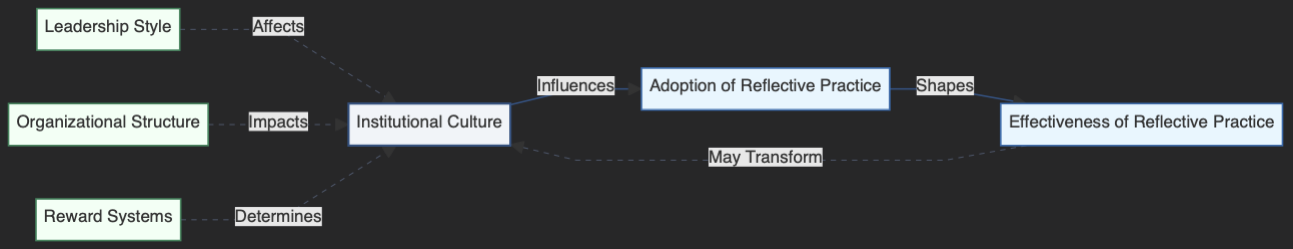
\includegraphics[width=6.72917in,height=\textheight]{image-20240920181655029.png}

  \textbf{Figure 12} shows the relationship between institutional
  culture and various organizational factors in shaping the adoption and
  effectiveness of reflective practice. Institutional culture (main
  concept, blue-gray) directly influences the adoption of reflective
  practice, which in turn shapes its effectiveness (process variables,
  blue). The effectiveness of reflective practice can potentially
  transform institutional culture, creating a feedback loop. Leadership
  style, organizational structure, and reward systems (outcome
  variables, green) indirectly impact institutional culture,
  contributing to its overall influence on reflective practice.
\item
  \textbf{Reflective Practice and Innovation}: \\
  Examine the relationship between regular engagement in reflective
  practice and academic innovation, including new teaching methods,
  research breakthroughs, and interdisciplinary collaborations.
\item
  \textbf{Ethical Considerations}: \\
  Explore the ethical implications of promoting reflective practice in
  academic settings, including issues of privacy, pressure to conform,
  and potential misuse of personal insights.
\item
  \textbf{Policy Impact}: \\
  Assess how national and institutional policies can be designed to
  effectively support and incentivize reflective practice among
  academics.
\end{enumerate}

By addressing these research directions, we can develop a more
comprehensive understanding of how reflective practice can be
effectively implemented and sustained in academic settings, particularly
in the context of Chinese higher education. This knowledge will be
crucial for developing evidence-based strategies to support early career
academics and enhance the quality of higher education more broadly.

\hypertarget{7-conclusion}{%
\subsection{7. Conclusion}\label{7-conclusion}}

This study has explored the potential of reflective practice as a
strategy for early career academics in Chinese universities to navigate
the complex challenges they face in their professional lives. Our
research, based on in-depth interviews with 22 early career academics
and a survey of 150 respondents across 30 Chinese universities, has
yielded several key insights:

\begin{enumerate}
\def\labelenumi{\arabic{enumi}.}
\item
  \textbf{Effectiveness of Reflective Practice}: Our findings suggest
  that structured reflection can be a powerful tool for early career
  academics, helping them to better integrate teaching and research,
  manage work-related anxiety, and navigate institutional pressures.
  However, the effectiveness of reflective practice is moderated by
  institutional culture, individual disposition, and disciplinary
  background.
\item
  \textbf{Balancing Teaching and Research}: Reflective practice appears
  to be particularly beneficial in helping academics find synergies
  between their teaching and research responsibilities. Those who
  engaged in regular reflection reported higher satisfaction with their
  ability to balance these often competing demands.
\item
  \textbf{Managing Academic Anxiety}: Our study revealed a correlation
  between engagement in reflective practice and lower levels of
  work-related anxiety. This suggests that reflection may serve as a
  coping mechanism in the high-pressure environment of Chinese academia.
\item
  \textbf{Navigating Institutional Pressures}: While reflective practice
  was seen as helpful in maintaining personal autonomy and purpose, its
  effectiveness in addressing systemic issues was limited. This
  highlights the need for complementary institutional and policy reforms
  to fully address the challenges faced by early career academics.
\item
  \textbf{Disciplinary Differences}: Our research uncovered significant
  variations in the adoption and perceived usefulness of reflective
  practice across different academic disciplines. This underscores the
  importance of developing discipline-specific approaches to promoting
  and implementing reflective practice.
\end{enumerate}

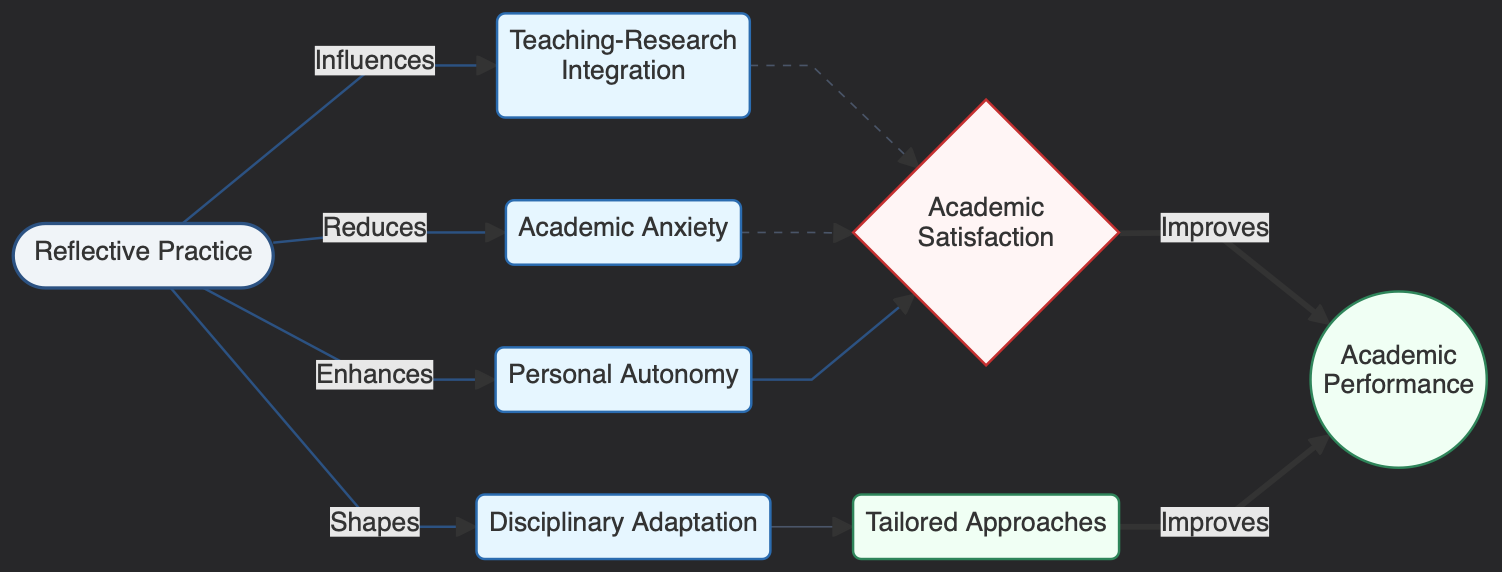
\includegraphics[width=7.82292in,height=\textheight]{image-20240920181655048.png}

\textbf{Figure 13} illustrates how reflective practice influences
academic performance through multiple pathways. Reflective practice
(main concept, blue-gray) directly impacts several process variables,
including teaching-research integration, academic anxiety, personal
autonomy, and disciplinary adaptation (process variables, blue). These
relationships are represented by thick solid arrows, indicating that
these are the primary pathways of influence from reflective practice.
Additionally, academic anxiety, teaching-research integration, and
personal autonomy affect academic satisfaction (mediator variable,
pink), shown by thin dashed arrows, suggesting that these are more
indirect mechanisms. Disciplinary adaptation influences tailored
approaches, which then indirectly contribute to academic performance.

This diagram illustrates the key findings of our study, showing how
reflective practice influences various aspects of academic life and
ultimately contributes to improved academic performance.

\hypertarget{implications-for-practice-and-policy}{%
\subsubsection{Implications for Practice and
Policy}\label{implications-for-practice-and-policy}}

Based on our findings, we propose the following recommendations:

\begin{enumerate}
\def\labelenumi{\arabic{enumi}.}
\item
  \textbf{For Early Career Academics}:

  \begin{itemize}
  \item
    Develop a structured approach to reflective practice, incorporating
    it into daily or weekly routines.
  \item
    Use reflection to align personal values with professional goals and
    activities.
  \item
    Seek out mentors or peer groups to engage in collective reflection
    and support.
  \end{itemize}
\item
  \textbf{For Institutional Leaders}:

  \begin{itemize}
  \item
    Provide training and resources on reflective practice for early
    career academics.
  \item
    Create institutional spaces and times for reflection, such as
    regular workshops or retreats.
  \item
    Recognize and reward reflective practice as part of professional
    development.
  \end{itemize}
\item
  \textbf{For Policy Makers}:

  \begin{itemize}
  \item
    Consider incorporating reflective practice into national frameworks
    for academic development.
  \item
    Fund research on the long-term impacts of reflective practice on
    academic careers and institutional performance.
  \item
    Develop policies that balance quantitative metrics with qualitative
    assessments of academic work, allowing space for reflection and
    innovation.
  \end{itemize}
\end{enumerate}

\hypertarget{future-directions}{%
\subsubsection{Future Directions}\label{future-directions}}

While this study provides valuable insights, it also highlights the need
for further research. Key areas for future investigation include:

\begin{itemize}
\item
  Longitudinal studies to track the long-term impact of reflective
  practice on academic careers.
\item
  Cross-cultural comparisons to understand how reflective practice might
  be adapted for different cultural contexts.
\item
  Investigation of how different types of institutions can effectively
  implement and support reflective practice.
\item
  Development of quantitative measures to assess the impact of
  reflective practice on various aspects of academic performance and
  well-being.
\end{itemize}

In conclusion, reflective practice offers a promising strategy for early
career academics in Chinese universities to navigate the challenges of
their professional environment. However, its effectiveness is contingent
on supportive institutional structures and individual commitment to the
reflective process. As the Chinese higher education system continues to
evolve, balancing the drive for international recognition with the need
to nurture sustainable academic careers will be crucial. Reflective
practice, while not a panacea, offers one pathway towards achieving this
balance.

By fostering a culture of reflection and continuous improvement, Chinese
universities can potentially enhance the quality of their teaching and
research, improve the well-being of their faculty, and ultimately
strengthen their position in the global academic community. However,
this will require a concerted effort from individual academics,
institutional leaders, and policymakers to create an environment that
values and supports reflective practice as an integral part of academic
life.

\hypertarget{references}{%
\subsection{\texorpdfstring{\textbf{References}}{References}}\label{references}}

Åkerlind, G.S. (2003). Growing and developing as a university teacher --
variation in meaning. \emph{Studies in Higher Education, 28}(4),
375--390. \url{https://doi.org/10.1080/0307507032000122242}

Boyer, E. L. (1990). \emph{Scholarship Reconsidered: Priorities of the
Professoriate}. New Jersey: The Carnegie Foundation for the Advancement
of Teaching, Princeton University Press.

Wang, A. (2022). Breaking an Eagle and Pick-up artists in a Chinese
Context. \emph{Acta Asiatica Varsoviensia}, (34), 357-375.

de Certeau, M. (1984). \emph{The practice of everyday life.} Berkeley,
CA: The University of California Press.

Diamond, R. M. (2002). Defining Scholarship for the Twenty-first
Century. \emph{New Directions for Teaching and Learning, 2002}(90),
73-80. \url{https://doi.org/10.1002/tl.57}

Dreier, O. (1999). Personal trajectories of participation across
contexts of social practice. \emph{Outlines, 1}(1), 5--32.
\url{https://doi.org/10.7146/ocps.v1i1.3841}

Evans, R. (2007). Comments on Shulman, Golde, Bueschel, and Garabedian:
Existing practice is not the template. \emph{Educational Researcher,}
\emph{36}(9), 553-559. \url{https://doi.org/10.3102/0013189X07313149}

Gibbs, P., Costley, C., Armsby, P., \& Trakakis, A. (2007). Developing
the ethics of worker researchers through phronesis. \emph{Teaching in
Higher Education, 12}(3), 365--375.
\url{https://doi.org/10.1080/13562510701278716}

Johnston, R. (1998). The University of the Future: Boyer Revisited.
\emph{Higher Education,} \emph{36}(3), 253-272.
\url{https://doi.org/10.1023/A:1003264528930}

Kalleberg, R. (2000). Universities: Complex bundle institutions and the
projects of enlightenment. In F. Engelstad, G., Brochmann, R.,
Kalleberg, A. Leira, \& L. Mjøset (Eds.), \emph{Comparative perspectives
on universities and production of knowledge} (pp. 219--257). Stamford,
CT: JAI Press.

Liu, B. N. (2015). A Study of University Teachers' Working Time.
\emph{Research on Open Education, 21}(2), 56-62. (In Chinese)

Cornford, I. R. (2002). Reflective teaching: Empirical research findings
and some implications for teacher education. \emph{Journal of Vocational
education and Training}, \emph{54}(2), 219-236.

Räsänen, K. (2009). Understanding academic work as practical activity -
and preparing (business‐school) academics for praxis?
\emph{International Journal for Academic Development, 14}(3), 185-195.
\url{https://doi.org/10.1080/13601440903106502}

Bullough, R. V., \& Hall‐Kenyon, K. M. (2011). The call to teach and
teacher hopefulness. \emph{Teacher Development}, \emph{15}(2), 127-140.

Schön, D. A. (2018). \emph{Reflective Practitioners: How Professional
Workers Think in Action.} (L. Q. Xia, Trans.). Beijing: Beijing Normal
University Press. (Original work published 1984 )

The Propaganda Department of the Party Committee. (2020, July 29). Zheng
Qiang, Secretary of the Party Committee of the school, was interviewed
by the Voice of China "News with Views" program.
\url{http://www2017.tyut.edu.cn/info/1027/18155.htm?from=singlemessage}
(In Chinese)

Foucault, M. (2023). Discipline and punish. In Social theory re-wired
(pp. 291-299). Routledge.

Wankat, P. C. (2002). \emph{The effective, eficient professor: Teaching,
scholarship and service.} Boston: Allyn and Bacon.

Müller, R. (2019). Racing for what? Anticipation and acceleration in the
work and career practices of academic life science postdocs. In
\emph{The Social Structures of Global Academia} (pp. 162-184). Routledge
.

Berg, L. D., Huijbens, E. H., \& Larsen, H. G. (2016). Producing anxiety
in the neoliberal university. \emph{The Canadian Geographer/le géographe
canadien}, \emph{60}(2), 168-180.

Boyer, E. L. (1990). Scholarship reconsidered: Priorities of the
professoriate. Princeton University Press, 3175 Princeton Pike,
Lawrenceville, NJ 08648 .

\end{document}
